% Template file for an a0 landscape poster.
% Written by Graeme, 2001-03 based on Norman's original microlensing
% poster.
%
% See discussion and documentation at
% <http://www.astro.gla.ac.uk/users/norman/docs/posters/> 
%
% $Id: poster-template-landscape.tex,v 1.2 2002/12/03 11:25:46 norman Exp $


% Default mode is landscape, which is what we want, however dvips and
% a0poster do not quite do the right thing, so we end up with text in
% landscape style (wide and short) down a portrait page (narrow and
% long). Printing this onto the a0 printer chops the right hand edge.
% However, 'psnup' can save the day, reorienting the text so that the
% poster prints lengthways down an a0 portrait bounding box.
%
% 'psnup -w85cm -h119cm -f poster_from_dvips.ps poster_in_landscape.ps'

\documentclass[a0]{a0poster}
% You might find the 'draft' option to a0 poster useful if you have
% lots of graphics, because they can take some time to process and
% display. (\documentclass[a0,draft]{a0poster})
\input defs
\pagestyle{empty}
\setcounter{secnumdepth}{0}
\renewcommand{\familydefault}{\sfdefault}
\newcommand{\QED}{~~\rule[-1pt]{8pt}{8pt}}\def\qed{\QED}

\renewcommand{\reals}{{\mbox{\bf R}}}

% The textpos package is necessary to position textblocks at arbitary 
% places on the page.
\usepackage[absolute]{textpos}

\usepackage{fleqn,psfrag,wrapfig,tikz}

\usepackage[papersize={38in,28in}]{geometry}

% Graphics to include graphics. Times is nice on posters, but you
% might want to switch it off and go for CMR fonts.
\usepackage{graphics}


% we are running pdflatex, so convert .eps files to .pdf
%\usepackage[pdftex]{graphicx}
%\usepackage{epstopdf}

% These colours are tried and tested for titles and headers. Don't
% over use color!
\usepackage{color}
\definecolor{Red}{rgb}{0.9,0.0,0.1}

\definecolor{bluegray}{rgb}{0.15,0.20,0.40}
\definecolor{bluegraylight}{rgb}{0.35,0.40,0.60}
\definecolor{gray}{rgb}{0.3,0.3,0.3}
\definecolor{lightgray}{rgb}{0.7,0.7,0.7}
\definecolor{darkblue}{rgb}{0.2,0.2,1.0}
\definecolor{darkgreen}{rgb}{0.0,0.5,0.3}

\renewcommand{\labelitemi}{\textcolor{bluegray}\textbullet}
\renewcommand{\labelitemii}{\textcolor{bluegray}{--}}

\setlength{\labelsep}{0.5em}


% see documentation for a0poster class for the size options here
\let\Textsize\normalsize
%\def\Head#1{\noindent\hbox to \hsize{\hfil{\LARGE\color{bluegray} #1}}\bigskip}
\def\Head#1{\noindent{\LARGE\color{bluegray} #1}\bigskip}
\def\LHead#1{\noindent{\LARGE\color{bluegray} #1}\bigskip}
\def\Subhead#1{\noindent{\large\color{bluegray} #1}\bigskip}
\def\Title#1{\noindent{\VeryHuge\color{Red} #1}}


% Set up the grid
%
% Note that [40mm,40mm] is the margin round the edge of the page --
% it is _not_ the grid size. That is always defined as 
% PAGE_WIDTH/HGRID and PAGE_HEIGHT/VGRID. In this case we use
% 23 x 12. This gives us three columns of width 7 boxes, with a gap of
% width 1 in between them. 12 vertical boxes is a good number to work
% with.
%
% Note however that texblocks can be positioned fractionally as well,
% so really any convenient grid size can be used.
%
\TPGrid[40mm,40mm]{23}{12}      % 3 cols of width 7, plus 2 gaps width 1

\parindent=0pt
\parskip=0.2\baselineskip

\begin{document}

% Understanding textblocks is the key to being able to do a poster in
% LaTeX. In
%
%    \begin{textblock}{wid}(x,y)
%    ...
%    \end{textblock}
%
% the first argument gives the block width in units of the grid
% cells specified above in \TPGrid; the second gives the (x,y)
% position on the grid, with the y axis pointing down.

% You will have to do a lot of previewing to get everything in the 
% right place.

% This gives good title positioning for a portrait poster.
% Watch out for hyphenation in titles - LaTeX will do it
% but it looks awful.
\begin{textblock}{23}(0,0)
\Title{The Title of the Project}
\end{textblock}

\begin{textblock}{23}(0,0.6)
{
\LARGE
Firstname Lastname
}

{
\Large
\color{bluegray}
\emph{Optimization Class Project. MIPT}
}
\end{textblock}


% Uni logo in the top right corner. A&A in the bottom left. Gives a
% good visual balance, but you may want to change this depending upon
% the graphics that are in your poster.
%\begin{textblock}{2}(0,10)
%Your logo here
%%\includegraphics{/usr/local/share/images/AandA.epsf}
%\end{textblock}

%\begin{textblock}{2}(21.2,0)
%Another logo here
%%\resizebox{2\TPHorizModule}{!}{\includegraphics{/usr/local/share/images/GUVIu/GUVIu.eps}}
%\end{textblock}


\begin{textblock}{7.0}(0,1.5)

\hrule\medskip
\Head{Introduction}\\
Many approaches to solving regression problems with hierarchical structures 
(\eg, Yuan \& Lin; Meier, van de Geer, B\"uhlmann; Jacob, Obozinski, Vert)
Lorem ipsum dolor sit amet, consectetur adipisicing elit, sed do eiusmod tempor incididunt ut labore et dolore magna aliqua. Ut enim ad minim veniam, quis nostrud exercitation ullamco laboris nisi ut aliquip ex ea commodo consequat. Duis aute irure dolor in reprehenderit in voluptate velit esse cillum dolore eu fugiat nulla pariatur. Excepteur sint occaecat cupidatat non proident, sunt in culpa qui officia deserunt mollit anim id est laborum.

\medskip
\hrule\medskip
\Head{Group lasso}\\
One approach is the \emph{group lasso}:
\[
\begin{array}{ll}
\mbox{minimize} & f(x) + \lambda \sum_{i=1}^N \|x_i\|_2
\end{array}
\]
\ie, like lasso, but require groups of variables to be zero or not
\begin{itemize}\itemsep=12pt
\item also called $\ell_{1,2}$ mixed norm regularization
\end{itemize}

\medskip
\hrule\medskip
\Head{Structured group lasso}\\
Another approach is the \emph{structured group lasso}:
\[
\begin{array}{ll}
\mbox{minimize} & f(x) + \sum_{i=1}^N \lambda_i \|x_{g_i}\|_2
\end{array}
\]
where $g_i \subseteq [n]$ and $\mathcal G = \{g_1, \dots, g_N\}$
\begin{itemize}\itemsep=12pt
\item like group lasso, but the groups can overlap arbitrarily
\item particular choices of groups can impose `structured' sparsity
\item \eg, topic models, selecting interaction terms for (graphical) models,
    tree structure of gene networks, fMRI data
\item generalizes to the \textbf{composite absolute penalties family}:
\[
r(x) = \|(\|x_{g_1}\|_{p_1}, \dots, \|x_{g_N}\|_{p_N})\|_{p_0}
\]
\end{itemize}

\medskip
\hrule\medskip
\Head{Hierarchical selection}\\
\begin{center}
\begin{tikzpicture}
[dot/.style={rectangle,draw=black,fill=white,inner sep=5pt,minimum size=5pt}]
\node[dot,draw=orange,thick] at (0,10) (n1) {1};
\node[dot] at (-3,8) (n2) {2};
\node[dot,draw=orange,thick] at (3,8) (n3) {3};
\node[dot] at (-3,6) (n4) {4};
\node[dot,draw=orange,thick] at (1.5,6) (n5) {5};
\node[dot] at (4.5,6) (n6) {6};
\draw[->] (n1) -- (n2);
\draw[->] (n1) -- (n3);
\draw[->] (n2) -- (n4);
\draw[->] (n3) -- (n5);
\draw[->] (n3) -- (n6);
\end{tikzpicture}
\end{center}

\begin{itemize}\itemsep=8pt
    \item $\mathcal G = \{ \{4\}, \textcolor{orange}{\{5\}}, \{6\}, \{2,4\}, 
        \textcolor{orange}{\{3,5,6\}}, \textcolor{orange}{\{1,2,3,4,5,6\} \}}$
\item nonzero variables form a rooted and connected subtree
    \begin{itemize}
        \item if node is selected, so are its ancestors
        \item if node is not selected, neither are its descendants
    \end{itemize}
\end{itemize}

\end{textblock}

\begin{textblock}{7.0}(8,1.5)
\hrule\medskip
\Head{Algorithm}\\
We solve this problem using an ADMM lasso implementation:
\begin{verbatim}
prox_f = @(v,rho) (rho/(1 + rho))*(v - b) + b;
prox_g = @(v,rho) (max(0, v - 1/rho) - max(0, -v - 1/rho));

AA = A*A';
L  = chol(eye(m) + AA);

for iter = 1:MAX_ITER
    xx = prox_g(xz - xt, rho);
    yx = prox_f(yz - yt, rho);

    yz = L \ (L' \ (A*(xx + xt) + AA*(yx + yt)));
    xz = xx + xt + A'*(yx + yt - yz);
  
    xt = xt + xx - xz;
    yt = yt + yx - yz;
end
\end{verbatim}

\medskip
\hrule\medskip
\Head{Line search}\\
If $L$ is not known (usually the case), can use the following line search:

\noindent\rule[-5pt]{.8\textwidth}{0.4pt}
{\footnotesize
\begin{tabbing}
    {\bf given} $x^k$, $\lambda^{k-1}$, and parameter $\beta \in (0,1)$. \\*[\smallskipamount]
    Let $\lambda := \lambda^{k-1}$. \\*[\smallskipamount]
    {\bf repeat} \\
    \qquad \= 1.\ Let $z := \prox_{\lambda g}(x^{k} - \lambda \nabla f(x^{k}))$. \\
    \> 2.\ {\bf break if} $f(z) \leq \hat{f}_{\lambda}(z, x^{k})$. \\
    \> 3.\ Update $\lambda := \beta \lambda$. \\*[\smallskipamount]
    {\bf return} $\lambda^{k} := \lambda$, $x^{k+1}:=z$.
\end{tabbing}}
\noindent\rule[10pt]{.8\textwidth}{0.4pt}

typical value of $\beta$ is $1/2$, and 
\[
\hat{f}_\lambda(x,y) = f(y) + \nabla f(y)^T (x - y) + 
(1/2\lambda)\|x - y\|_2^2
\]

\medskip
\hrule\medskip
\Head{Convergence proof}\\
Lorem ipsum dolor sit amet, consectetur adipisicing elit, sed do eiusmod tempor incididunt ut labore et dolore magna aliqua. Ut enim ad minim veniam, quis nostrud exercitation ullamco laboris nisi ut aliquip ex ea commodo consequat. Duis aute irure dolor in reprehenderit in voluptate velit esse cillum dolore eu fugiat nulla pariatur. Excepteur sint occaecat cupidatat non proident, sunt in culpa qui officia deserunt mollit anim id est laborum.

\end{textblock}

\begin{textblock}{7.0}(16,1.5)

\hrule\medskip
\Head{Numerical example}\\
Consider a numerical example with $f(x) = \|Ax - b\|_2^2$
with $A \in \reals^{10 \times 100}$ and $b \in \reals^{10}$.
Entries of $A$ and $b$ are generated as independent samples from
a standard normal distribution.
Here, we have chosen $\lambda$ using cross validation.

\medskip
\hrule\medskip
\Head{Results}\\
On this numerical example, the ADMM method converges quickly.
We give two realizations corresponding to different parameters $A$ and $b$.
\begin{center}
\psfrag{k}[t][b]{$k$}
\psfrag{fbest - fmin}[b][t]{$f_\mathrm{best}^{(k)} - f^\star$}
\psfrag{noise-free realize}{noise-free case}
\psfrag{realize1}{realization 1}
\psfrag{realize2}{realization 2}
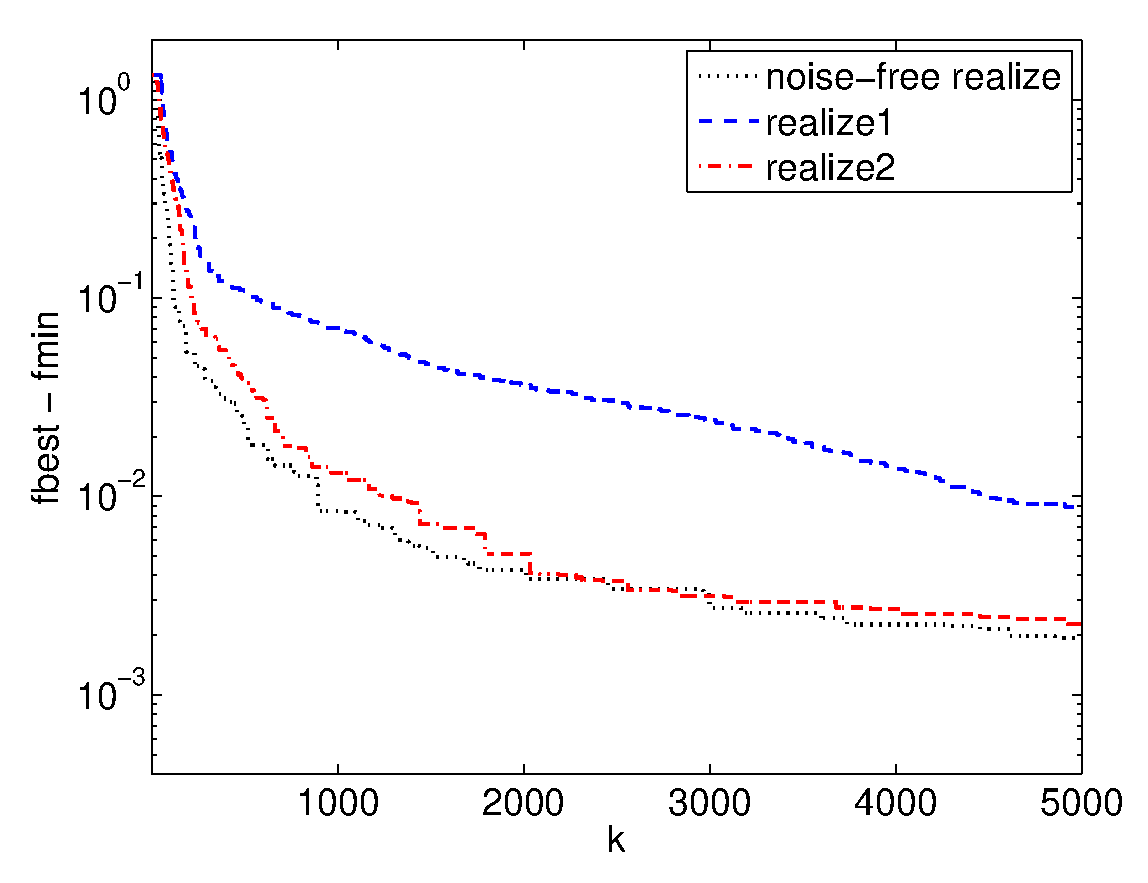
\includegraphics[width=0.9\textwidth]{figures/pwl_error_fbest_realize.eps}
\end{center}

\medskip
\hrule\medskip
\Head{Conclusion}\\
Lorem ipsum dolor sit amet, consectetur adipisicing elit, sed do eiusmod tempor incididunt ut labore et dolore magna aliqua. Ut enim ad minim veniam, quis nostrud exercitation ullamco laboris nisi ut aliquip ex ea commodo consequat. Duis aute irure dolor in reprehenderit in voluptate velit esse cillum dolore eu fugiat nulla pariatur. Excepteur sint occaecat cupidatat non proident, sunt in culpa qui officia deserunt mollit anim id est laborum.

\medskip
\hrule\medskip
\Head{Acknowledgements}\\
This material is based upon work supported by the
X Fellowship and my mom.

\end{textblock}

\end{document}
